\documentclass{../style/sig-alternate}

\usepackage{here}

%----------- マクロ ----------
%数式番号を節毎に分けてリセットする
\def\theequation{\thesection.\arabic{equation}}
  \makeatletter
  \@addtoreset{equation}{section}
  \makeatother
%図番号を節毎に分けてリセットする
\makeatletter
 \renewcommand{\thefigure}{%
   \thesection.\arabic{figure}}
  \@addtoreset{figure}{section}
\makeatother
%表番号を節毎に分けてリセットする
\makeatletter
 \renewcommand{\thetable}{%
   \thesection.\arabic{table}}
  \@addtoreset{table}{section}
\makeatother

\makeatletter
 \let\@copyrightspace\relax
 \makeatother

\begin{document}

\title{SLSTC at the NTCIR-12 STC Task}

\numberofauthors{5}
\author{
% You can go ahead and credit any number of authors here,
% e.g. one 'row of three' or two rows (consisting of one row of three
% and a second row of one, two or three).
%
% The command \alignauthor (no curly braces needed) should
% precede each author name, affiliation/snail-mail address and
% e-mail address. Additionally, tag each line of
% affiliation/address with \affaddr, and tag the
% e-mail address with \email.
%
% 1st. author
\alignauthor
Hiroto Denawa\\
       \affaddr{Waseda University}\\
       \email{hi\_denawa@fuji.waseda.jp}
% 2nd. author
\alignauthor
Tomoaki Sano\\
       \affaddr{Waseda University}\\
       \email{tonosamoaki@asagi.waseda.jp}
\and  % use '\and' if you need 'another row' of author names
% 3rd. author
\alignauthor
Yuta Kadotami\\
       \affaddr{Waseda University}\\
       \email{kdtm-783640@ruri.waseda.jp}
% 4th. author
\alignauthor
Sosuke Kato\\
       \affaddr{Waseda University}\\
       \email{sow@suou.waseda.jp}
%\and  % use '\and' if you need 'another row' of author names
% 5th. author
\alignauthor
Tetsuya Sakai\\
       \affaddr{Waseda University}\\
       \email{tetsuyasakai@acm.org}
}

\maketitle

\begin{abstract}
The SLSTC team participated in the Short Text Conversation (STC) task at NTCIR-12 Task.
This minority report describes our approach to solving the STC problem and will discuss the official results.
\end{abstract}

\section*{Team Name}
SLSTC

\section*{Subtasks}
Short Text Conversation (Japanese)

\keywords{STC,HNN,Word2Vec,pagerank,word co-occurrence network}

\section{Introduction}

SLSTC (The Sakai Laboratory, Waseda University) participated in the
Japanese subtask of the STC task.
This paper briefly describes our approaches,
and reports on the official results.

Table \ref{tab:run_list}  shows the list of runs that we submitted to the STC Japanese subtask.
In Section~\ref{sec:methods}, we describe the algorithms we employed
to generate these runs.
In Section~\ref{sec:results}, we discuss the official results of our runs.
Finally, in Section~\ref{sec:conclusions}, we conclude this paper
and lists up future work items.

\begin{table}[h!]
  \centering
  \caption{the list of runs}
  \label{tab:run_list}
  \begin{tabular}{|c|} \hline
     run name \\ \hline
     SLSTC-J-R1 \\ \hline
     SLSTC-J-R2 \\ \hline
     SLSTC-J-R3 \\ \hline
  \end{tabular}
\end{table}

\section{Methods}
\label{sec:methods}

\subsection{SLSTC-J-R1}

This experiment can be divided in following 4 parts: 1st parts of generating distributed representation, 2nd of processing train data, 3rd of training and 4th of applying system learned and evaluation. In this section details of these are shown below.

\subsubsection{Distributed Representation Generating Module}

There is a tool for generate distributed representation of words called Word2Vec\cite{word2vec}.
Word2Vec is announced by Google in 2013 and attracted researchers’ attention all over the world.
Input a corpus, Word2Vec generates vectors for each word in the corpus.
Words which have close meaning have close vectors to each other.
In this research, Wikipedia in Japanese and Nicopedia (Niconico Daihyakka in Japanese) corpus were used to generate distributed representation, to apply to somehow casual representation in sentences.

\subsubsection{Train Data Processing Module}

Dataset is provided by NTCIR-12 STC Task.
From this dataset, 427200 pairs of post tweet and reply tweet were obtained (maybe some were deleted).
For each tweet in this dataset, morpheme analysis was done by using MeCab\cite{mecab}.
Then, for each tweet, vector representation of it was calculated as follows.
$ i $ th morpheme in tweet $ t $ was defined as  and its vector (distributed) representation is noted as $ {\bf w_{i,t}} $.
The vector representation of tweet $ t $ is calculated by:

\begin{eqnarray}
 {\bf t} = \sum_{i=1}^{|t|} tfidf(w_{i,t}) \cdot {\bf w_{i,t}} \cdot f(t,i)
\end{eqnarray}

Note that $ f(t,i) = e^{\frac{|l|}{i}} $ if $ i $ th morpheme in $ t $ is content word and  if otherwise.
This is to emphasize weight of content words.

\subsubsection{Learning Module}

In this research, process to make valid reply for given post is considered as a translation by Hierarchical Neural network (HNN) , which has 3 layers.
In this part, weight matrices in the HNN is learned by Error Back Propagation method\cite{bahman}.
The parameters used in this part are shown in table \ref{tab:hnn_parameters} below.
Note  stands for the sigmoid function .

\begin{table}[h!]
  \centering
  \caption{Parameters for learning}
  \label{tab:hnn_parameters}
  \begin{tabular}{|c|c|} \hline
     {\bf Parameters} & {\bf Value} \\ \hline
     Dimension of input layer & 200 \\ \hline
     Dimension of hidden layer & 100 \\ \hline
    Dimension of output layer & 200 \\ \hline
    Activity function to hidden & $ \sigma ( x ) $ \\ \hline
    Activity function to output & $ 2 \sigma ( x ) - 1 $ \\ \hline
    Learning efficiency $ \eta $ & $ 1.0 \times 10^{-4} $ \\ \hline
    Error threshold & $ 1.25 \times 10^{-2} $ \\ \hline
  \end{tabular}
\end{table}

This model is tested in 3-cross evaluation method.
All data were divided into 3 groups and tested in the scheme shown in table \ref{tab:testing_scheme} below.

\begin{table}[h!]
  \centering
  \caption{Training and testing scheme}
  \label{tab:testing_scheme}
  \begin{tabular}{|c|c|c|c|} \hline
     {\bf Experiment No.} & 1 & 2 & 3 \\ \hline
     {\bf Group No.} & & & \\ \hline
     0 & \multicolumn{2}{|c|}{Train} & Test \\ \hline
    1 & Test & \multicolumn{2}{|c|}{Train} \\ \hline
    2 & Train & Test & Train \\ \hline
  \end{tabular}
\end{table}

\subsubsection{Applying and Evaluating Module}
\label{sec:applying}

For each posts in each test case, five reply candidates, which has from 1st to 5th smallest error to its output are suggested.

\begin{figure}[h!]
 \begin{center}
  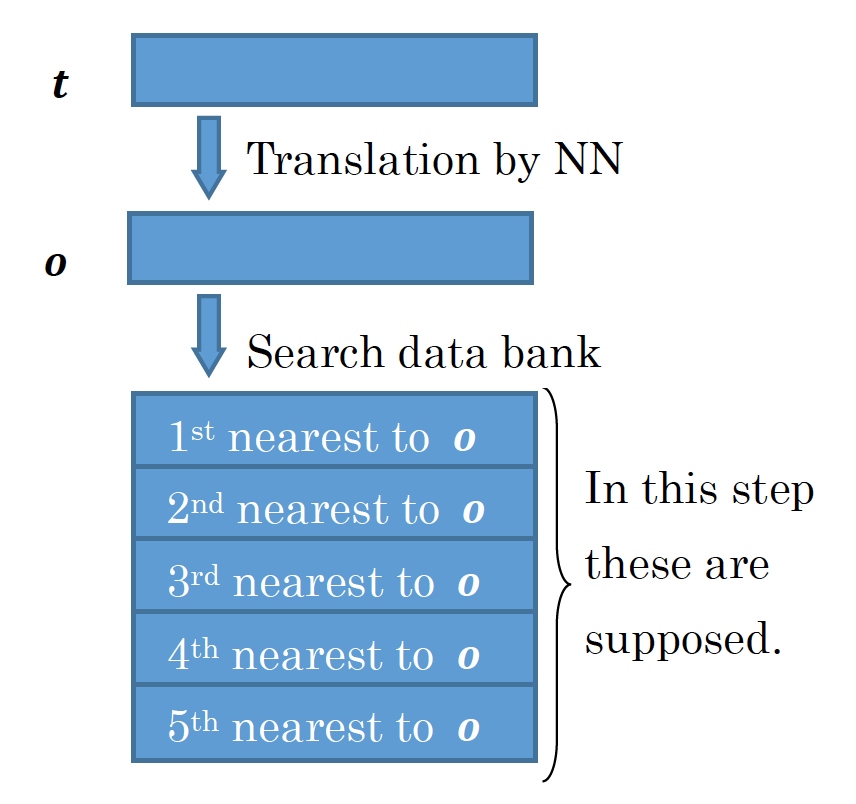
\includegraphics[width=120mm,bb=0 0 616 579]{../img/peter_fig01.png}
  \end{center}
  \caption{description of step}
  \label{fig:applying}
\end{figure}

\subsection{SLSTC-J-R2 and SLSTC-J-R3}
We adopt a method that using a word co-occurrence network.
This method has following 3 parts:
\begin{enumerate}
    \item Making Network
    \item Extracting Subnetwork
    \item Output Rank Result
\end{enumerate} 

\subsubsection{Making Network}
In this part, we make a word co-occurrence network from pairs of post tweets and reply tweet.
As we have already told in the previous section, the data has 427200 tweets. 
First, we analyze morphenom against all tweet pairs by MeCab. Then we extract pair of sets of noun words from each pair as \((W_{p}, W_{r})\). Wp or Wr contains a ordered word set which means faster word appear faster in the original tweet. And set \(V\) as an union of all pairs.

\begin{enumerate}
    \item \(W_{p} = (\omega_{p1}, \omega_{p2}, ... \omega_{pi} ... \omega_{pn}) \)
    \item \(W_{r} = (\omega_{r1}, \omega_{r2}, ... \omega_{ri} ... \omega_{rn}) \)
    \item \(P = \{W | W \in \bigcup W_{p} \wedge W \in \bigcup W_{r}\}\)
    \item \(V = \{\omega | \omega \in W \wedge W \in P\} \)
\end{enumerate}

Using V as nodes, we make a directed graph. We make a path from the first word in some tweet to the next word in the tweet and from each word in \( W_{p} \) to all words in \(W_{r} \).

\begin{eqnarray}
\begin{split}
E = &\{(\omega_{1}, \omega_{2}) | \omega_{1}\in W_{p} \lor \omega_{2}\in W_{r}\}\\
&\cup \{(\omega_{pi}, \omega_{p(i+1)}) | 0 < i < n-1\}\\
&\cup \{(\omega_{ri}, \omega_{r(i+1)}) | 0 < i < n-1\}
\end{split}
\end{eqnarray}


At last a word co-occurrence network G is defined like below:

\begin{eqnarray}
G := (V,E)
\end{eqnarray}

This word network shows what word likely appear next to some word. In other words, it shows that how wrods close to each other. So, it represents word distribution which contains topic distribution.

\subsubsection{Extracting Subnetwork}
Test tweet data is same as the data used in RUN1. As well as previous part, we extract set of noun words from each test tweet as \(W_{t} = (\omega_{t1}, \omega_{t2}, ... \omega_{ti} ... \omega_{tn})\).
In this part, we extract subnetwork $G'_{i}$ which contains \(\omega_{ti}\) from $G$.
If wti exists in V, pick up all nodes which is next to wti.

\begin{eqnarray}V'_{i} = \omega_{ti} \cup \{\omega_{e} |  (\omega_{ti}, \omega_{e}) \in E\}\end{eqnarray}
\begin{eqnarray}E'_{i} = \{(\omega_{ti}, \omega_{e}) | (\omega_{ti}, \omega_{e}) \in E\} \end{eqnarray}

Finaly, we get a subnetwork G' like below:

\begin{eqnarray}G'_{i} = (V'_{i}, E'_{i})\end{eqnarray}

\(G' = \bigcup G'_{i}\) represents potential topics of expected replies.

\subsubsection{Output Rank Result}
In this part, we get results for each $W_{t}$ using subnetworks we get previous part. We add score to each possible reply using the score like tf-idf and pagerank\cite{pagerank}.

First, we calculate pagerank for each word in $W_{t}$. With $E(\omega_{k})$, which is the number of edges that has $\omega_{k}$ as the start node, a pagerank is calculated. And $d$ is some parameter set $0.9$ in our experiment.

\begin{eqnarray}PR(\omega_{ti}) = \frac{(1-d)}{N} + \sum_{\omega_{k}\in V'_{i}} d(\frac{PR(\omega_{k})}{E(\omega_{k})})\end{eqnarray}

Then, we calculate final score with tf-idf like score. $P'$ is a set of tweets which concludes $\omega_{ti}$. 

\begin{eqnarray}P'_{ij} = \{W_{j} | W_{j} \in P \wedge \omega_{ti} \in W_{j}\}\end{eqnarray}

And, we define $df$ as the number of tweets in $P'$, $N$ as the number of tweets in $P$, $l$ as the number of word in $W_{i}$, and tc as how many $\omega_{ti}$ appear in $W_{i}$.

\begin{enumerate}
    \item $df_{i} = n(P'_{ij})$
    \item $N = n(P)$
    \item $idf = \log_{10} \frac{N}{df} + 1$
    \item $l_{i} = n(W_{j})$
    \item $tc_{i} = n(\{\omega | \omega = \omega_{ti} \wedge \omega \in W_{j}\})$
\end{enumerate}

Finaly, the score is caculated like below:

\begin{eqnarray}Score(W_{j}) = \sum_{i} \frac{l-tc+1}{l} idf PR(\omega_{ti})\end{eqnarray}

Following this score, our system return the rank list of $W_{j}$ against each test data $W_{t}$.

\subsubsection{Two types of system}

  We analyzed result of this run. We considered that continuous ``w'' was noise. So, we remove morpheme include continuous ``w''.
  Our submition of Run2 is type of not removed ``w'', and Run3 is type of removed ``w''.



\section{Official Results and Discussions}
\label{sec:results}
Table 1 shows the results of our systems, the maximam score of the other systems and the minimum score of the other systems. 
"ACX-Y" means that X indicates what score is regarded as true output and Y indicates the range of the acceptable rank. For example, "AC12-1" means that the outputs scored 1 or 2 and having top rank is evaluated.

From the results, our systems seem not to work. To know what kind of trouble occures in our system, we analyzed details of the results.


Figure 1 shwos what tweet appeared frequently as a possible reply. This figure indicates our system provide a nealy same set of tweets as possible replies. So, our results doesn't relate to inputs strongly. Something is wrong with our scoring algorithms. For, we analyzed the structure of subnetworks and its pagerank, TF and IDF.


Figure 2 and 3 show what words are enabled as a input and what words appear in a subnetwork for each input.
The accuracy of both outputs are relatively low: 0.04 for the former one, 0.16 for the latter one in "AC12-5". But, the words in the former result seems to be connected to inputs. For example, in input words, "各駅停車" and "神戸三宮" are words related to transpotation facility. And, in the subnetwork, "バスターミナル" is also a word related to transpotation facility. Why is accuracy low? We think this is caused by too many words in each subnetwork. Too many words in a subnetwork makes too low pagerank for each word. That means all scores of the output tweets reflect TF and IDF directly.
On the other hands, the words in the latter result seem not to be connected to inputs. To begin with, the words "さんが", "プラス", "して" seem to indicate no topics. The system failed to analyze morphenom appropriately.

So, in both cases, the results of our system doesn't reflect input topics. Instead, the data only about the frequency of words effects the results. So, our system outputs almost the same set of tweets.

\section{Conclusions and Future Work}
\label{sec:conclusions}
We made systems with Neural Network or word co-occurrence network. In this task, we didn't get good results but few conclusions like below.

For the system using a word co-occurrence network, we need to improve accuracy of morpheme analysis and the mothod for generating subnetwork.
In particular, for analyzing morphenom, we will try to improve the accuracy of dictionary or to handle newer or unknown words appropriately. And, for decreasing tne number of edges of nodes in each subnetwork, we will try to define something weight of the edge or to set strict condition on generating edges in a word co-occurrence network.

\begin{thebibliography}{99}

%\bibitem{sakai} Sakai, T., Shang, L., Lu, Z. and Li, H.: Topic Set Size Design with the Evaluation Measures for Short Text Conversation, AIRS 2015, LNCS 9460, pp.1-13, 2015.
\bibitem{word2vec} Google Word2Vec, https://code.google.com/p/word2vec/
\bibitem{mecab} MeCab, http://taku910.github.io/mecab/
\bibitem{bahman} Bahman Kermanshahi, Construction and Application of Neural Network,Shokodo
\bibitem{pagerank} Sergey Brin, Rajeev Motwani, and Terry Winograd. What can you do with a
web in your pocket. Data Engineering Bulletin, Vol. 21, pp. 37-47, 1998.

\end{thebibliography}


\end{document}
